% presentation source for the git-wizard presentation
% build with the make file

\documentclass{beamer}
\mode<presentation>
\usetheme{Montpellier}
\usecolortheme{rose}

% preamble {{{

% packages {{{
\usepackage[normalem]{ulem}
\usepackage{listings}
% packages }}}

% defs {{{
\lstset{% set defaults
    basicstyle=\ttfamily,
    stringstyle=\ttfamily,
    showstringspaces=false
}
\lstnewenvironment{shell}
    {\lstset{language=sh}}
    {}
\hypersetup{% for links
    colorlinks,
    linkcolor=,
    urlcolor=blue
}
\theoremstyle{example}
\newtheorem{exercise}{Exercise}
\newcommand{\xkcd}[1]{\href{https://xkcd.com/#1}{xkcd/#1}}
% defs }}}

% metadata {{{
\title{Git Wizard 101}
\subtitle{Pearl Hacks}
% \author{D. Ben Knoble \\ \texttt{ben.knoble@gmail.com}}
\author{\href{https://benknoble.github.io}{D. Ben Knoble}}
% \urladdr[D. Ben Knoble]{https://benknoble.github.io} % or this
\institute{UNC Chapel Hill}
\date{23 February 2019}
% metadata }}}

% preamble }}}

\begin{document} % {{{

\frame{\titlepage}

\part{Getting Started}
\frame{\partpage}
\frame{\tableofcontents[part=1]}

\section{Ground Rules}
\begin{frame}{Ground Rules}
    \begin{itemize}
        \item Introduce yourself with name and pronouns
        \item Respect others' pronouns
        \item There are no dumb questions
        \item Help your neighbor when you can
        \item Have a good time!
    \end{itemize}
\end{frame}

\section{Introductions}
\begin{frame}{About Me}
    \begin{itemize}
        \item He/Him/His
        \item Senior (CS, French, Math), soon-to-be M.S. student
        \item \href{https://github.com/benknoble}{@benknoble} on GitHub
        \item<2-> Conversationally proficient in French, D\&D, puns
        \item<3-> And, of course, all things \texttt{git}
    \end{itemize}
\end{frame}

\begin{frame}{What We Will \emph{Not} Be Doing}
    \begin{columns}
        \column{0.5\textwidth}
        \begin{figure}
            
\includegraphics[scale=0.4]{img/git}
            \caption{\xkcd{1597}}
        \end{figure}

        \column{0.5\textwidth}
        \begin{itemize}
            \item Memorizing magic commands
            \item Learning the (beautiful) model behind \texttt{git}
        \end{itemize}
    \end{columns}
\end{frame}

\section{Setup}
\begin{frame}{Required setup}
    \begin{enumerate}[<+->]
        \item
            \href{https://git-scm.com/book/en/v2/Getting-Started-Installing-Git}
            {\texttt{git}}
        \item
            \href{https://github.com}
            {GitHub account}
        \item \href{https://desktop.github.com}
            {GitHub Desktop} [be sure to sign in with GitHub!]
        \item \href{https://github.com/benknoble/git-wizard-code/fork}{Fork}
            and
            \href{https://help.github.com/en/desktop/contributing-to-projects/cloning-a-repository-from-github-desktop}{clone}
            the
            \href{https://github.com/benknoble/git-wizard-code}{starter code}
    \end{enumerate}
\end{frame}

\begin{frame}{Other notes}
    \begin{itemize}
        \item GitHub Desktop is a \texttt{git} \emph{client}---other programs
            exist that allow you to use \texttt{git}, too
        \item GitHub is not \texttt{git}; it hosts projects that use
            \texttt{git}
    \end{itemize}
\end{frame}

\part{The Magic of \texttt{git}}
\frame{\partpage}
\frame{\tableofcontents[part=2]}

\section{First Steps with \texttt{git}}
\begin{frame}{We Don't Want To Do This}
    \begin{columns}
        \column{0.5\textwidth}
        \begin{figure}
            
\includegraphics[scale=0.4]{img/documents}
            \caption{\xkcd{1459}}
        \end{figure}

        \column{0.5\textwidth}
        \begin{itemize}
            \item Because we are software engineers and artists
            \item Because there is a better way
        \end{itemize}
    \end{columns}
\end{frame}

\begin{frame}{Instead}
    We commit.

    \begin{definition}[Commit]
        A snapshot in time of a project's \emph{content} that knows what came
        before it.
    \end{definition}
\end{frame}

\begin{frame}{How?}
    \begin{definition}[Commit]
        A snapshot in time of a project's \emph{content} that knows what came
        before it.
    \end{definition}
    \begin{enumerate}
        \item Make changes
        \item Add files
        \item Commit
        \item (Push to update a remote)
    \end{enumerate}
\end{frame}

\begin{frame}[fragile]{Lumos: Your First \sout{Spell} Commit}
    {Not the time for \emph{commitment} problems}
    \begin{exercise}[Make a commit]
        \begin{enumerate}
            \item Create \texttt{yourname.txt}
            \item Place your name in it
            \item Click commit
            \item Push to your fork
        \end{enumerate}
    \end{exercise}
\end{frame}

\begin{frame}{Lumos: Your First \sout{Spell} Commit}
    \begin{figure}
        
\includegraphics[scale=0.4]{img/create_ben}
        \caption{Create \texttt{ben.txt}}
    \end{figure}
\end{frame}

\begin{frame}{Lumos: Your First \sout{Spell} Commit}
    \begin{figure}
        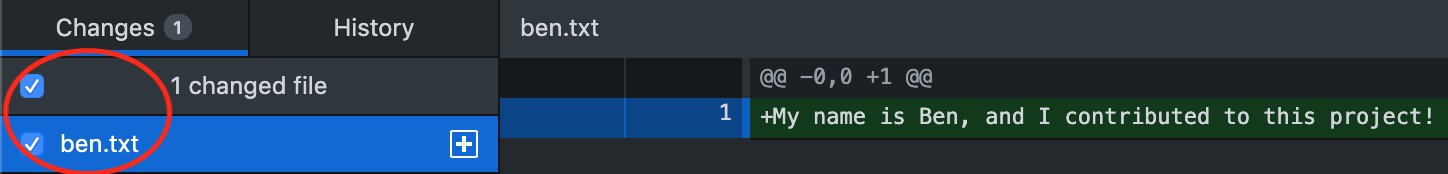
\includegraphics[scale=0.4]{img/add_ben}
        \caption{Add \texttt{ben.txt}}
    \end{figure}
\end{frame}

\begin{frame}{Lumos: Your First \sout{Spell} Commit}
    \begin{figure}
        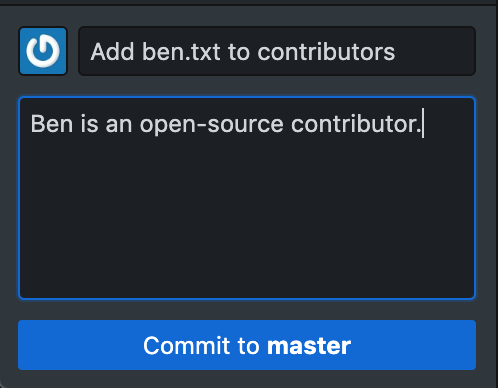
\includegraphics[scale=0.4]{img/commit_ben}
        \caption{Commit}
    \end{figure}
\end{frame}

\begin{frame}{Lumos: Your First \sout{Spell} Commit}
    \begin{figure}
        
\includegraphics[scale=0.4]{img/history_ben}
        \caption{History}
    \end{figure}
\end{frame}

\begin{frame}{A Note about Messages}
    \begin{columns}
        \column{0.5\textwidth}
        \begin{figure}
            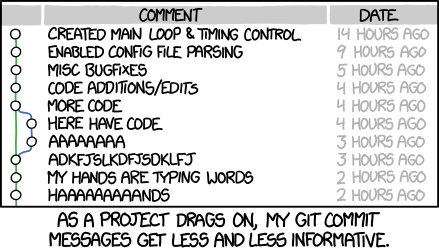
\includegraphics[scale=0.4]{img/git_commit}
            \caption{\xkcd{1296}}
        \end{figure}

        \column{0.5\textwidth}
        Our messages should summarize the what and describe the why.
        \href{https://tbaggery.com/2008/04/19/a-note-about-git-commit-messages.html}
        {Here's a good format to follow.}
    \end{columns}
\end{frame}

\section{Experimentation with the Multiverse}
\begin{frame}{Trying new things}
    How many of you have ever\dots
    \begin{itemize}[<+->]
        \item edited code?
        \item tried to undo your edits?
        \item tried several approaches to a problem, and had to use undo/redo?
    \end{itemize}
\end{frame}

\begin{frame}{Remember this?}
    \begin{figure}
        
\includegraphics[scale=0.4]{img/documents}
        \caption{\xkcd{1459}}
    \end{figure}
\end{frame}

\begin{frame}{Branches}
    Git's version of an experiment is called a \emph{branch}

    \begin{definition}[Branch]
        A pointer to a commit.
    \end{definition}

    Remember that a commit knows who it's parent is, so if I have a pointer to a
    commit---a branch---I have an entire \emph{branch} of history in the history
    tree.
\end{frame}

\begin{frame}{Why would I do this?}
    \begin{columns}
        \column{0.5\textwidth}
        \begin{figure}
            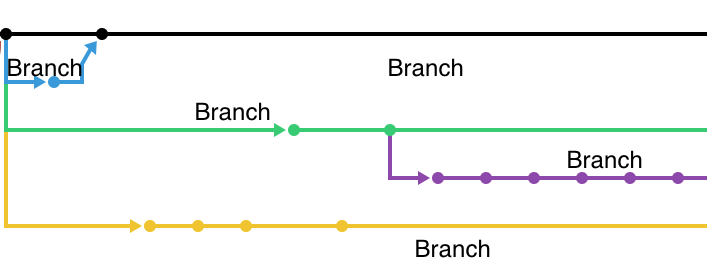
\includegraphics[scale=0.4]{img/branches}
            \caption{Some branches}
        \end{figure}

        \column{0.5\textwidth}
        \begin{itemize}
            \item to separate work on feature A from feature B
            \item to experiment without affecting the main code
            \item to make pretty graphs
        \end{itemize}
    \end{columns}
\end{frame}

\begin{frame}{Potions Class \& PPE\@: Experimenting Safely}
    Let's make a branch for a code experiment we want to do
    \begin{exercise}[Branching]
        \begin{enumerate}
            \item Use the Branch menu to create a new branch and switch to it
            \item Implement \texttt{add1} by changing \texttt{pass} to
                \texttt{return a + 1}
            \item Commit (you've seen this before!)
            \item Switch back to master and implement \texttt{sub1} the same way
            \item Commit
        \end{enumerate}
    \end{exercise}
\end{frame}

\begin{frame}{Creating a branch}
    \begin{columns}
        \column{0.5\textwidth}
        \begin{figure}
            
\includegraphics[scale=0.4]{img/branch_menu}
            \caption{Menu}
        \end{figure}

        \column{0.5\textwidth}
        \begin{figure}
            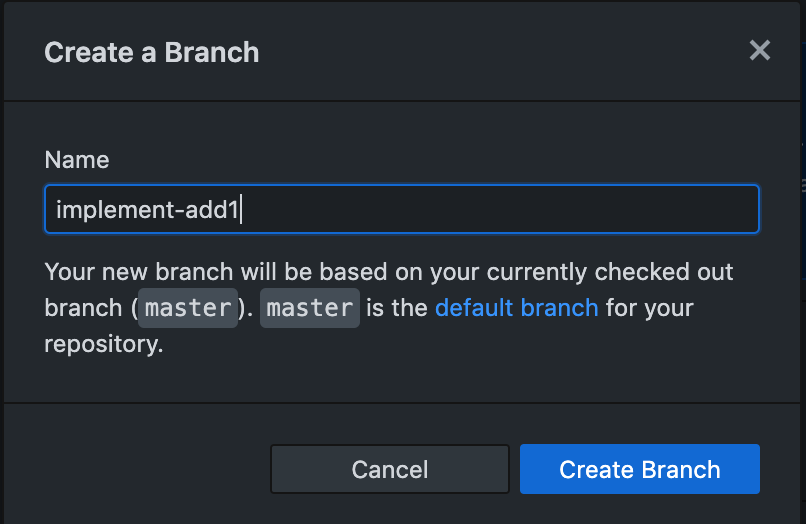
\includegraphics[scale=0.4]{img/create_branch}
            \caption{Naming a branch}
        \end{figure}
    \end{columns}
\end{frame}

\begin{frame}{Implementing \texttt{add1}}
    \begin{figure}
        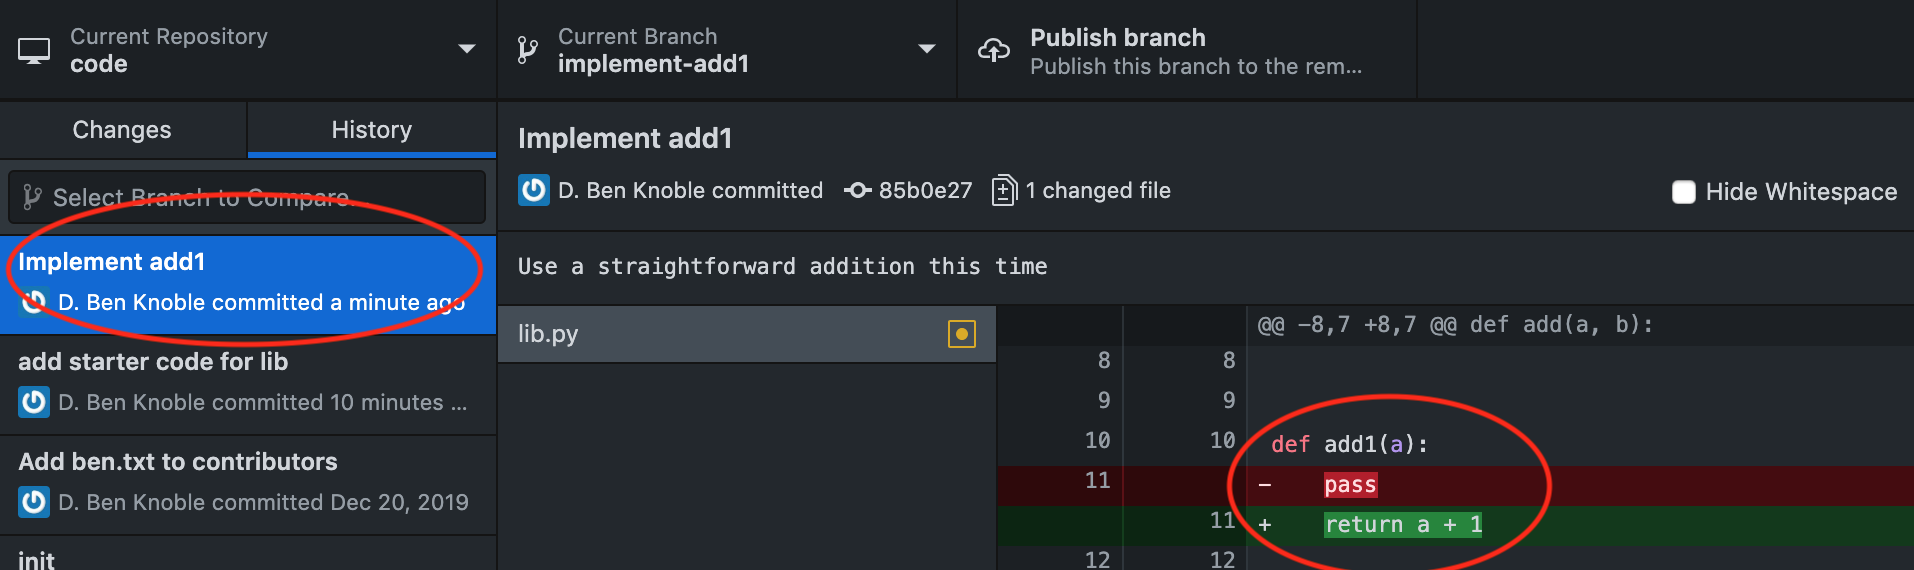
\includegraphics[scale=0.4]{img/add1}
        \caption{The \texttt{add1} commit}
    \end{figure}
\end{frame}

\begin{frame}{Implementing \texttt{sub1} back on master}
    \begin{figure}
        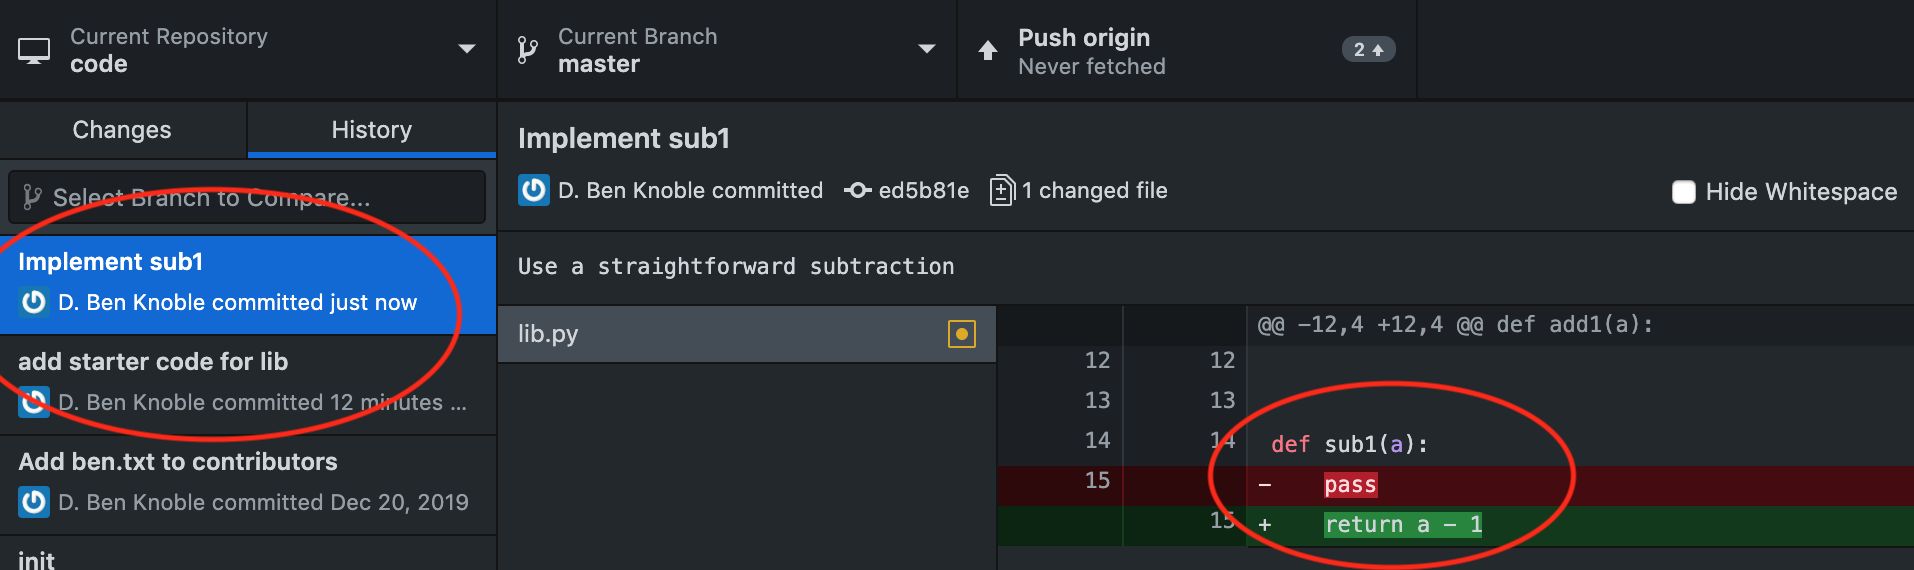
\includegraphics[scale=0.4]{img/sub1}
        \caption{The \texttt{sub1} commit}
    \end{figure}
\end{frame}

\begin{frame}{Comparing the history}
    \begin{figure}
        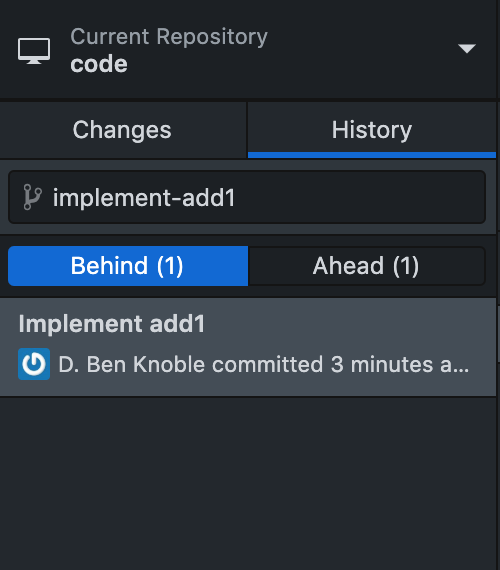
\includegraphics[scale=0.4]{img/comparing}
        \caption{Some commits on each branch}
    \end{figure}
\end{frame}

\begin{frame}[The experiment is a success: now what?]
\end{frame}

\section{Collaboration in a Distributed System}
\begin{frame}{Accio Code! Collaborating via Pull Requests}
\end{frame}

\section{Advanced: Dealing with Merge Conflicts}
\begin{frame}{Boggarts and Riddikulus: Merge Conflicts are \alert{not} Scary!}
\end{frame}

\part{Conclusion}
\begin{frame}{Conclusion}
    \begin{block}{Who Am I?}
    \end{block}
    \begin{block}{Summary}
    \end{block}
    \begin{block}{Resources}
    \end{block}
    \begin{block}{Reminders}
    \end{block}
    \begin{block}{Upcoming Wizard Classes}
    \end{block}
\end{frame}

% \appendix

\end{document} % }}}
